\documentclass{article}
\usepackage[utf8]{inputenc}

\title{COMP 138 RL: Data Efficiency Experiment}
\author{Tung Pham}

\usepackage{natbib}
\usepackage{graphicx}

\begin{document}

\maketitle

\section{Introduction}
In Viet Nam, there is a biggest holiday that we're all considered to be the
start of the New Year. It's the tradition that was influenced by the
colonization of China for thousands of years in our history. And that is Tet.
During this time, if you visit any household, you cannot miss the celebration,
the ceremony, food and concerts. But most importantly is a homemade casino.

Some believe that gambling for Tet is a test of fortune in the new coming lunar
year, some use it as a form of entertaining as it can be played with a large
group of people, while the kids consider it as a form to gain more lucky money.

As a Vietnamese myself, and as a kid, my family always enjoy 2 games of cards,
black jack and 13 (which we call it "go forward"). I was raise to not be a
gambler but in these occasion, I'm allowed to participate in blackjack as a form
of bonding time with my big family as it can be played in a big circle while my
dad and my uncles are gathering in the 13 game group.

But the issue with this is that, I always lose in blackjack! And I have no idea when or
should I hit. If I don't hit and got find out that the cards I'm holding is not
enough, I'll lose, if I hit, I go above 21 and busted. Occasionally, I win the game but
that's extremely rare.

Now that I have learned about reinforcement learning, it can be used
in this scenario to maximize my profit. However, what training mechanism should I follow?
N-step was a technique that balance the trade-off between traditional methods
like Monte Carlo and Temporal Difference. However, between n-step SARSA Off-policy and On-policy,
which is better in this problem?
In this experiment, I'll use 3 approaches to compare, an Off-Policy n-step SARSA with
control variates, a regular Off-policy n-step SARSA, and an On-policy n-step
SARSA. All methods utilize n-step algorithm as the base but have different
approaches to update the value of a state that the agent went through and were
capable of learning the target policy, $\pi$. The average estimated value
function will be reported with discussion for better understand the differences.

\section{Problem}
The problem is formulated with less rules and mainly focus on getting
to 21 and not busted. At each time step, the agent have 2 options: stick or hit.
If the agent decides to stick, the
dealer will reveal the remaining hand and begin drawing cards until their sum is
17 or above. However, if a hit, by either the agent or the dealer, result in a bust, the game immediately stop and
whoever bust is considered lost the game. As the number of episodes increase,
the agent has a 10\% chance of trying a random move to explore if there's any
other undiscovered pattern and that can leads to better profit.

The point values of the cards is as follows:
\begin{enumerate}
	\item Face cards (Jack, Queen, King) have 10 points
	\item Aces can be either 11 or 1 point.
	\item Numerical cards have a point value equal to their number.
\end{enumerate}

After both sides has finished hitting, if the value of both are the same, then
that counts as a draw. Whoever has a higher value hands wins the game.

In this problem, I'll only consider a single agent environment where there's
only the agent and the dealer. I'll assume an idealistic scenario where the cards are drawn from an infinite
deck which in theory guarantee randomness of hands in a deck whereas in reality, the deck has a
finite number of hands and therefore can be predicted if pay enough attention.

\section{Methodology}
\subsection{Environment}
In this work, the Gymnasium's BlackJack environment was used as it meets all of
our requirements of a simple and fundamental but robust enough to fully
represent the core functionality of the game.
\subsection{On-policy n-step SARSA}
On-policy N-step SARSA allows us to use N steps experience to update the Q value
and action selection. This allows better generalization than traditional
Temporal Difference approach as instead of using 1 single experience to update Q
value, N-step allows N steps to be taking into consideration when updating the Q
value. This therefore making a better judgement and action selection. As this is
updating as the agents experience the environment, it's faster and way more
efficient than traditional Monte Carlo approach. Figure \ref{fig:Figure1} illustrate the
algorithm that is used to implement this \citep{sutton_barton}.
\begin{figure}[!ht]
	\centering
	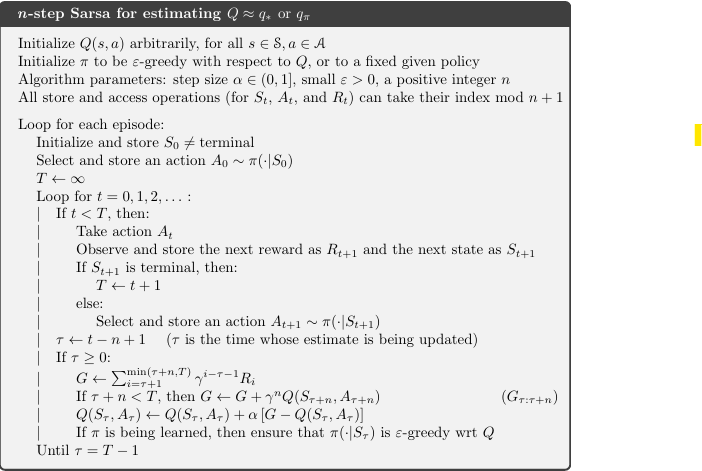
\includegraphics[scale=0.65]{./images/Figure 1.png}
	\caption{The on-policy n-step SARSA algorithm.}
	\label{fig:Figure1}
\end{figure}
The return value, G, is updated using the formula (7.1) of Sutton and Barton
\citep{sutton_barton} which is Monte Carlo updates extended to n-steps.
\[
	G_{t:t+n}=R_{t+1}+\gamma R_{t+2} + \dots +
	\gamma^{n-1}R_{t+n}+\gamma^nV_{t+n-1}(S_{t+n})
\]
And the state value estimation, Q, is updated using the formula (7.2).
\[
	V_{t+n}(S_t) = V_{t+n-1}(S_t)+\alpha[G_{t\:t+n} -
		V_{t+n-1}(S_t)]
\]

\subsection{Off-policy n-step SARSA}
However, just learning a single policy limits the exploration of the agents.
Therefore, an Off-policy was tested by trying to learn the optimal policy while
following another policy. This allows the agents to learn from many sources and
therefore, has more exploration capability than on-policy. As the problem of
BlackJacks tends to be different as time goes on due to randomness of the hands
give out. Figure \ref{fig:Figure6} notes the algorithm for Off-policy n-step SARSA.

\begin{figure}[!ht]
	\centering
	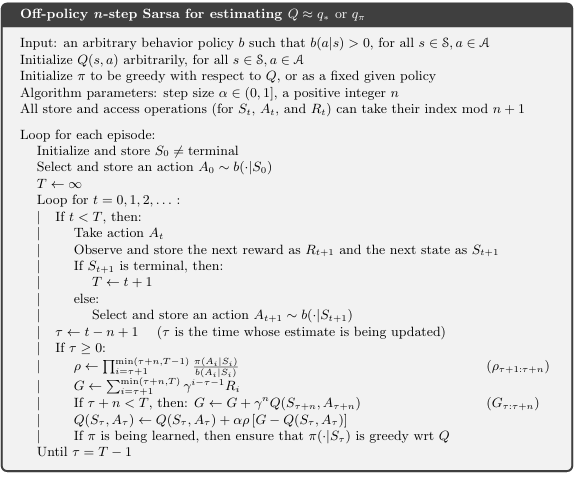
\includegraphics[scale=0.54]{./images/Figure 6.png}
	\caption{The off-policy n-step SARSA algorithm.}
	\label{fig:Figure6}
\end{figure}

In implementation, the state value, Q, is updated using the formula (7.9) of Sutton and Barton
\citep{sutton_barton}.
\[
	V_{t+n}(S_t) = V_{t+n-1}(S_t)+\alpha\rho_{t\:t+n-1}[G_{t\:t+n} -
		V_{t+n-1}(S_t)]
\]

where $0 \leq t < T$ and $\rho_{t\:t+n-1}$ denotes the importance sampling ratio
for n-steps, let $h = t + n$, which is defined as the ratio between the target policy and the behavior
policy\citep{sutton_barton}.
\[
	\rho_{t\:h} = \prod_{k=t}^{min(h, T-1)}\frac{\pi(A_k|S_k)}{b(A_k|S_k)}
\]

This importance sampling ratio allows the agents to correct the difference
between the behavior policy $b$, that generated the action, and the target policy
$\pi$.

The return value, G, update formula is following (7.1) of Sutton and Barton
\citep{sutton_barton} where it is a Monte Carlo update function that was
extended for n-steps return update\citep{sutton_barton}.
\[
	G_{t:t+n}=R_{t+1}+\gamma R_{t+2} + \dots +
	\gamma^{n-1}R_{t+n}+\gamma^nV_{t+n-1}(S_{t+n})
\]

Although this method is more generalized to the observation of the training
environment, there are a few draw back where in the return calculation, the
algorithm takes into account all the rewards that was seen which can introduce
high variance as there could potentially be a case of randomly exploration. This
can make the training unstable and slow. To tackle this problem, another
improvement could be made to this algorithm which is the control variates which
will be going over in the next section.
\subsection{Off-policy n-step SARSA with control variates}
To introduce the control variates into the calculation of the returns value, G,
formula (7.13) of Sutton and Barton was used \citep{sutton_barton}.

\[
  G_{t:h}=\rho_t(R_{t+1}+\gamma G_{t+1:h})+(1-\rho_t)V_{h-1}(S_t)
\]

However, according to Sutton and Barton, "For a conventional n-step method, the
learning rule to use in conjunction with (7.13) is the n-step TD update
(7.2)" \citep{sutton_barton}.
One observation is that because (7.13) has already include the importance
sampling ratio in the calculation of returns. Therefore, if (7.9) was used, it
would be duplicating the impact of the sampling ratio.

The second term in (7.13), $(1-\rho_t)V_{h-1}(S_t)$ is the control variate. This
term helps mitigate the shrinking behavior of the returns when $\rho_t$ is small
or even equals to zero. The results is a reduction in high variance that is occuring for the
standard n-step off-policy SARSA algorithm. This produce a more stable and
therefore faster for the agent to learn. 

\section{Experiment}
The implementation of the method can be found in train\_on.py file that is
included in the attached code. It's similar to Temporal Difference where we
start out with initializing Q to have arbitrary values for all actions for a
given state. In the context of this experiment, uniform distribution between $0$ and $1$ was used.
For consistency for comparison, the n value was kept fixed at $5$ steps
look back.

Due to the nature of randomness in the possible hands could have for hitting,
it's intuitive to value the later the same scale as the past experience.
Therefore, $0.9$, which is closed to $1$ was used through out all of the
experiments.

To also encourage the agent to try out something different once in a while, or
encourage exploring other options, $\epsilon$-greedy was used as the behavior
policy for the agents to follow. And $\epsilon = 0.1$ is chosen for the task as
high $\epsilon$ could leads to high exploration and less exploitation but we
still wants to follow the current policy that the agent learned.

\begin{figure}[h!]
	\centering
	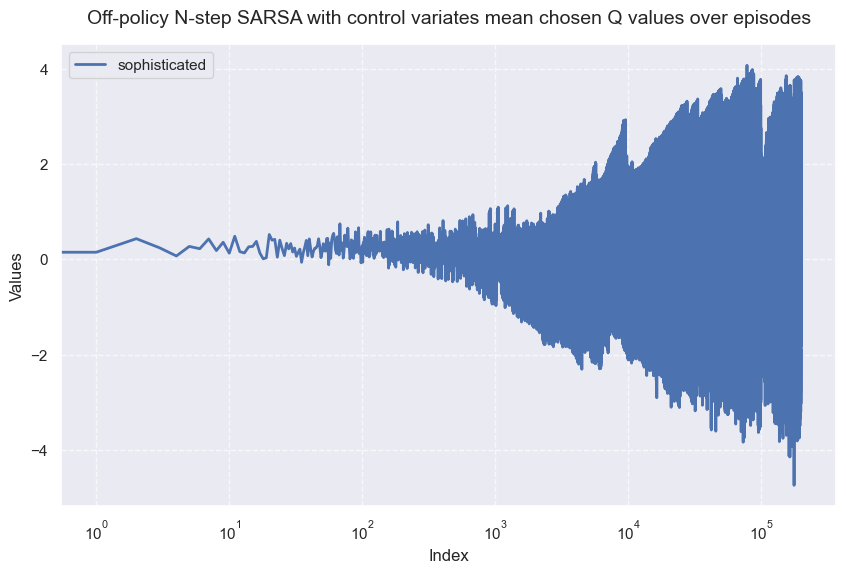
\includegraphics[scale=0.54]{./images/Figure 2.png}
	\caption{The off-policy N-Step SARSA with Control Variates mean chosen Q over
  episodes}
	\label{fig:Figure2}
\end{figure}

\begin{figure}[!ht]
	\centering
	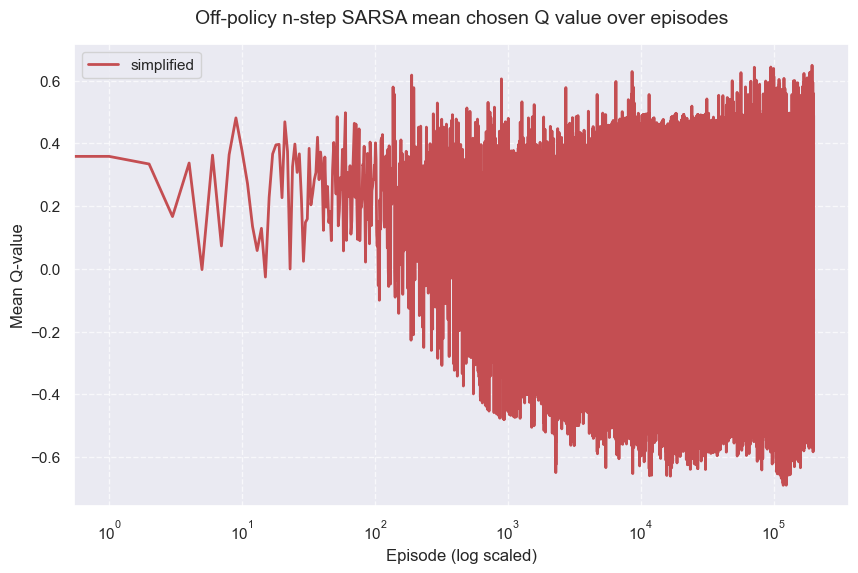
\includegraphics[scale=0.55]{./images/Figure 3.png}
	\caption{The off-policy N-Step SARSA mean chosen Q over
  episodes}
	\label{fig:Figure3}
\end{figure}

\begin{figure}[!ht]
	\centering
	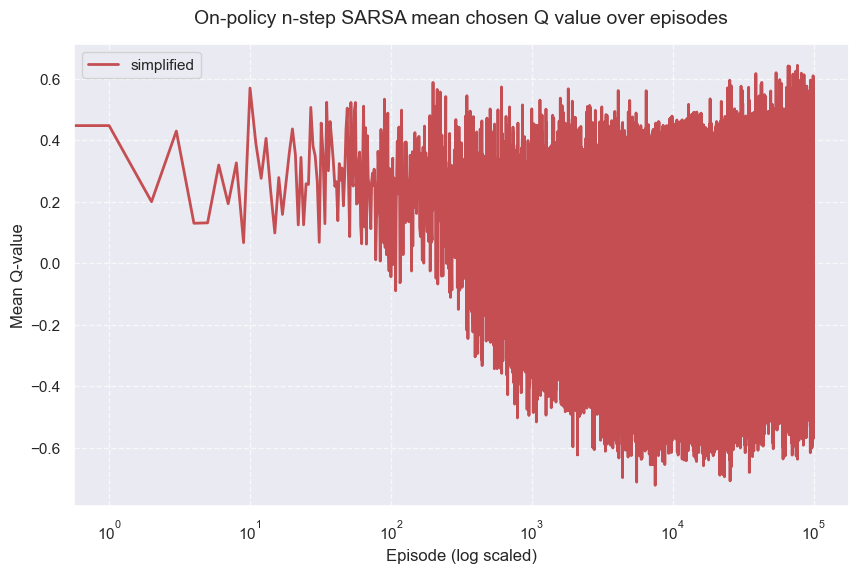
\includegraphics[scale=0.50]{./images/Figure 4.png}
	\caption{The on-policy N-Step SARSA mean chosen Q over
  episodes}
	\label{fig:Figure4}
\end{figure}

Each method is then run through 100,000 episodes and we record the average Q value
updated at each episode to see the pattern and impact of each method on
estimating the true value of each state. 

\section{Discussion}
Through the experiment above, we obtains Figure
\ref{fig:Figure2},
\ref{fig:Figure3}, and
\ref{fig:Figure4} which are
plots of mean Q value progression obtain for Off-policy n-step SARSA with control variates, regular
Off-policy n-step SARSA, and On-policy n-step SARSA respectively.

When comparing the on-policy plot with the off-policy plot, they seems to behave
the same way. They both starts out more stable whcih could also be because we're
plotting in log scale but as we increasing the number of episodes, there are
some more clear evidence of high variance in both approaches. Both begin to
establish high variance around  episode $10^2$ and from there, they established
jittering behavior between $0.4$ to $-0.6$. We then tried to look at the rewards
of the two approaches which can be seen in Figure \ref{fig:Figure7}
to inspect if there are any differences but none could be observed.

\begin{figure}[!ht]
	\centering
	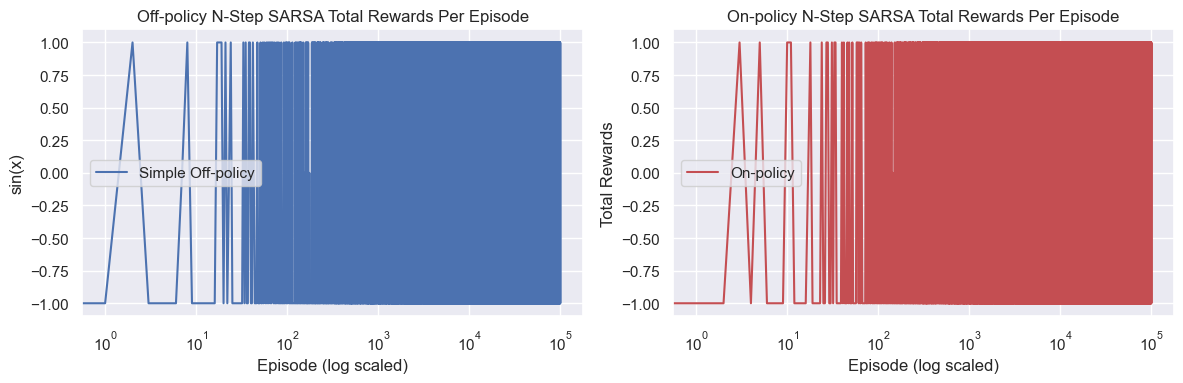
\includegraphics[scale=0.50]{./images/Figure 7.png}
	\caption{The total rewards in each episode of On-policy and Off-policy}
	\label{fig:Figure7}
\end{figure}

The values of both approaches all have a downward trends as the number of
episodes increases while still oscillate with the upper bound of $0.6$ and
converge to lower bound of $0.6$ around episode $10^4$. 
This is an indication that the more we gambled, we can still gain some profit,
however, we'll still lose some money along the way and is not a good way to make
money.

On the other hand, when comparing the Off-policy n-step SARSA with its control variates
variant, we can clearly see the improvement in terms of stability. While regular
N-Step struggles to be stable and have its Q value shrinking randomly
through out $100,000$ episodes. With control variates, however, the graph remains more
stable until around episode $10^3$ and the variance increased afterwards. This
promise an improvement in performance and we documented
the recorded training time in Figure
\ref{fig:Figure5}. We can observe
that the sophisticated agent with control variates $0.3$ second faster than the
on-policy variant and $1$ second faster than the traditional off-policy agent.
This improvement was not significant as there maybe some code redundancy or
unoptimized implementation which leads to this degraded performance.

\begin{figure}[!ht]
	\centering
	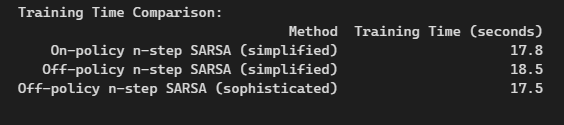
\includegraphics[scale=0.50]{./images/Figure 5.png}
	\caption{Total training time of each method}
	\label{fig:Figure5}
\end{figure}

\section{Conclusion}
In this experiment, we can again confirm on the fact that the more we gamble,
the more we're going to both lose and win money but the balance will remains
unchange in an idealistic world. In reality, it's not a good way to make money
by gambling as there are tricks behind the scene that we do not know of and this
will affects the profit that we got in returns.

We also saw that both on-policy and off-policy implementation perform the same 
on this problem of choosing action to take for BlackJack. While with control 
variates, it's clear that the variation in Q values is mitigated. However, 
the performance boost from this work remains minimal.


\bibliographystyle{plain}
\bibliography{references}
\end{document}
